\documentclass[aspectratio=169,11pt]{beamer}
% Plantilla del centro (base Madrid, paleta azul marino tipo pptx).
% babel/fontenc/inputenc/helvet/hyperref y el estilo los carga la propia plantilla.
% Para el look "pptx" (titulo sin barra) usa:  \usepackage[plano]{beamertemplate}
\usepackage{beamertemplate}
\usepackage{graphicx}
\usepackage{tikz}
\usepackage{url}
\usepackage[normalem]{ulem} 
\usepackage{epstopdf}

% Texto justificado en las diapositivas (beamer usa ragged right por defecto).
% OJO: NO parchear \frame con \apptocmd -> rompe el parseo de [allowframebreaks]{titulo}
% y hace desaparecer la barra del titulo. Se justifican las listas (que es casi todo el
% contenido) y, para el texto suelto, se activa \justifying al empezar cada frame.
\usepackage{ragged2e}
\usepackage{etoolbox}
\apptocmd{\itemize}{\justifying}{}{}
\apptocmd{\enumerate}{\justifying}{}{}
\apptocmd{\description}{\justifying}{}{}
\AtBeginEnvironment{frame}{\justifying}

\title[SSI -- Tema 1.1]{Presentación de la Asignatura}
\subtitle{Seguridad en Sistemas Informáticos --- Tema 1.1}
\author{José Luis Martínez}
\institute{Universidad de Castilla-La Mancha}
\date{Curso 2026/27}

% --- build reproducible / metadatos limpios ---
\pdfinfoomitdate=1
\pdftrailerid{}
\pdfsuppressptexinfo=-1

\begin{document}

\begin{frame}[plain]
  \titlepage
\end{frame}

\begin{frame}[allowframebreaks]{Presentación}
\small
\begin{itemize}
  \item Profesores
  \item Horarios
  \item Operativa
  \item Temario
  \item Evaluación
  \item Bibliografía
\end{itemize}
\end{frame}

\begin{frame}[allowframebreaks]{Profesores}
\small
\begin{itemize}
  \item José Luis Martínez
  \begin{itemize}
    \item Joseluis.martinez@uclm.es
    \item Despacho: 1.C.11
  \end{itemize}
  \item Cristina Olmedilla López
  \begin{itemize}
    \item Cristina.Olmedilla@alu.uclm.es
    \item Sala RAAP, i3a
  \end{itemize}
\end{itemize}
\end{frame}

\begin{frame}[allowframebreaks]{Profesores}
\small
\begin{itemize}
  \item Y, vosotros ?¿
  \begin{itemize}
    \item ¿Cómo os llamáis?
    \item ¿ Qué sabéis de ciberseguridad?
    \item ¿ Por qué elegisteis esta intensificación?
    \item ¿ Qué esperáis de esta asignatura?
    \item ¿ Qué habéis oído de ella de alumnos de otros años?
    \item ¿ Cuál es la asignatura que más os ha gustado de la carrera ?
  \end{itemize}
\end{itemize}
\end{frame}

\begin{frame}[allowframebreaks]{Horarios}
\small
\begin{itemize}
  \item Horario Teoría:
  \begin{itemize}
    \item Miércoles, de 13:05 a 14:35
    \item Jueves, de 11:35 a 13:05,
    \item Aula 1.5
  \end{itemize}
  \item Horario Laboratorio
  \begin{itemize}
    \item Viernes, de 13:05 a 14:35
    \item Aula 1.5
  \end{itemize}
\end{itemize}
\end{frame}

\begin{frame}[allowframebreaks]{Operativa}
\small
\begin{itemize}
  \item La asignatura está diseñada para impartirse un enfoque eminentemente práctico
  \item No hay lecciones magistrales como tal, el enfoque es como si fuera un taller.
  \begin{itemize}
    \item Quejas de: “el profesor no explica”
    \item Si hay pequeñas píldoras de explicación que preceden a la actividad práctica
  \end{itemize}
  \item Tenemos que:
  \begin{itemize}
    \item No hay PCs en las aulas
    \item El laboratorio sólo lo tenemos asignado una clase a la semana y la carga docente de la parte práctica es mucho mayor que la parte “teórica”
    \item Dependemos de un PC / portátil para seguir la asignatura
    \item El laboratorio que montamos y desarrollamos a lo largo del curso lo usaremos tanto para las clases, como la evaluación continua, \sout{como para el examen de laboratorio}
  \end{itemize}
  \item Opción Preferible:
  \begin{itemize}
    \item Trabajar en el aula con nuestros PCs / portátiles
  \end{itemize}
\end{itemize}
\end{frame}

\begin{frame}[allowframebreaks]{Temario}
\small
\begin{itemize}
  \item ¿qué vamos a aprender?
\end{itemize}
\begin{center}
\includegraphics[width=0.35\textwidth]{img/s7_2.jpg}\end{center}
\end{frame}

\begin{frame}[allowframebreaks]{Temario}
\small
\begin{itemize}
  \item Bloque 1: Introducción a la seguridad:
  \begin{itemize}
    \item Tema 1.1: Presentación de la Asignatura
    \item Tema 1.2: Introducción a la seguridad Informática y de la Información
    \item Tema 1.3: Montaje de un laboratorio de Ciberseguridad
  \end{itemize}
  \item Bloque 2: Recopilación de Información:
  \begin{itemize}
    \item Tema 2.1: Footprinting \& Open Source Intelligence (OSINT)
    \item Tema 2.2: Escaneo y técnicas de evasión
    \item Tema 2.3: Enumeración
  \end{itemize}
\end{itemize}
\end{frame}

\begin{frame}[allowframebreaks]{Temario}
\small
\begin{itemize}
  \item Bloque 3: Ataques de Acceso:
  \begin{itemize}
    \item Tema 3.1: Ataques a las credenciales
    \item Tema 3.2: Ingeniería Social
    \item Tema 3.3: Hacking con metasploit
    \item Tema 3.4: Denegación de Servicio (DoS)
  \end{itemize}
  \item Bloque 4: Pentesting:
  \begin{itemize}
    \item Tema 4.1: Hacking Web: Ataques Client-side
    \item Tema 4.2: Hacking Web: Ataques Server-side
    \item Tema 4.3: Hacking BBDD: Inyecciones SQL
  \end{itemize}
\end{itemize}
\begin{itemize}
  \item Bloque 5: Post Explotación:
  \begin{itemize}
    \item Tema 5.1: Meterpreter
    \item Tema 5.2: Hacking Manual \& Escalada de Privilegios
  \end{itemize}
\end{itemize}
\end{frame}


% Diagrama a pantalla completa (full-bleed) con TikZ: cubre TODA la diapositiva sin
% el margen que deja \paperwidth en el cuerpo y sin avisos de overfull. Se usa el PDF
% (mas robusto que EPS con pdfLaTeX: sin epstopdf/shell-escape).
\begin{frame}[plain]
\begin{tikzpicture}[remember picture,overlay]
  \node at (current page.center)
    {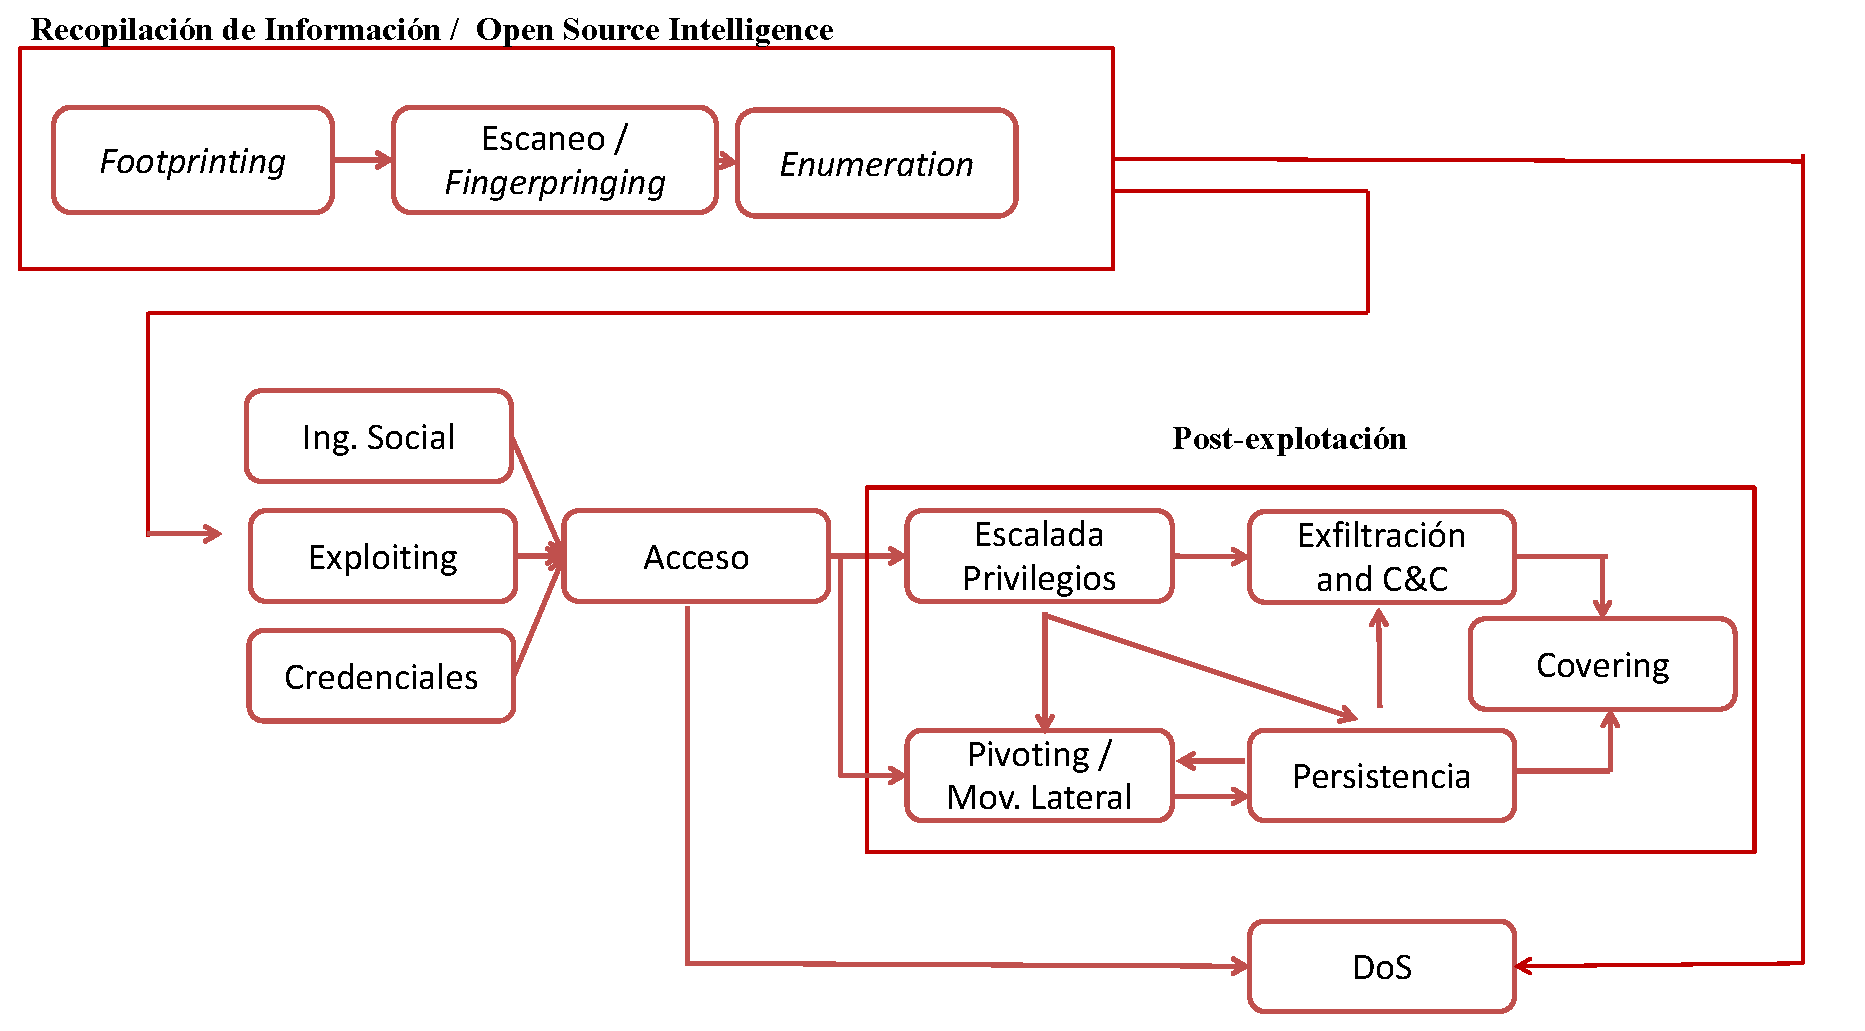
\includegraphics[width=\paperwidth,height=\paperheight,keepaspectratio]{img/Diagrama.pdf}};
\end{tikzpicture}
\end{frame}

\begin{frame}[allowframebreaks]{Temario}
\small
\begin{itemize}
  \item Esta imagen es un diagrama de flujo que representa el proceso de:
  \begin{itemize}
  \item Auditoria
  \item Hacking ético
  \item Pentesting
  \item Ejercicios Red Team
  
\end{itemize}
\item Las sesiones presenciales serán eminentemente de carácter práctico. Se pueden seguir con el profesor
  \item Además, se requiere de un trabajo autónomo del alumno. Las técnicas se aprenden practicando, no observando
  \end{itemize}
\end{frame}

\begin{frame}[allowframebreaks]{Evaluación}
\small
\begin{itemize}
  \item Se desglosará en las siguientes TRES partes (Eval, Exa y Extra):
  \item 1) EVAL (50\% de la nota final) :
  \begin{itemize}
    \item La asistencia a clase NO será obligatoria
    \item Evaluación de 3-4 hitos a lo largo del curso.
  \end{itemize}
  \item 2) EXA (50\% de la nota final):
  \begin{itemize}
    \item Examen Final Teórico: 25\% (Nota Mínima: 4)
    \item Examen Final Práctico: 25\% (Nota Mínima: 4)
  \end{itemize}
  \item 3) Puntos Extra (10\% de la nota final)
  \begin{itemize}
    \item Retos, pruebas, etc
  \end{itemize}
  \item Nota final = [Teoría + Prácticas]+Extra
  \item ESTE ES EL MODO DE EVALUACIÓN CONTÍNUA
\end{itemize}
\end{frame}

\begin{frame}[allowframebreaks]{Evaluación}
\small
\begin{itemize}
  \item Se desglosará en las siguientes DOS partes (teoría y práctica):
  \item 1)Teoría (50\% de la nota final) :
  \begin{itemize}
    \item La asistencia a clase NO será obligatoria
    \item Examen Final: 50\% (Nota Mínima: 4)
  \end{itemize}
  \item 2)Prácticas (50\% de la nota final):
  \begin{itemize}
    \item La asistencia a clase NO será obligatoria
    \item Examen Final : 50\% (Nota Mínima: 4)
  \end{itemize}
  \item Nota final = Teoría + Prácticas
  \item ESTE ES EL MODO DE EVALUACIÓN CONVENCIONAL
  \item MI RECOMENDACIÓN: SEGUIR LA ASIGNATURA ONLINE MEDIANTE EL MODO EVALUACIÓN CONTÍNUA
\end{itemize}
\end{frame}

\begin{frame}[allowframebreaks]{Evaluación}
\small
\begin{itemize}
  \item Examen Final de Teoría Ordinario/Extraordinario:
  \begin{itemize}
    \item Cuestiones cortas relativas a los conceptos, técnicas, ejercicios, herramientas vistos a lo largo del curso
  \end{itemize}
  \item Examen Final de Prácticas Ordinario/Extraordinario:
  \begin{itemize}
    \item Consistirá en realizar, algún(os) caso(s) similar(es) a los desarrollados en las clases con la ayuda de las diferentes Herramientas y técnicas usadas en clases.
    \item Se permitirá utilizar todo el material que se considere oportuno sin conexión a internet \sout{ChatGPT}
    \item \sout{Importante, tener en vuestro PC/portátil el laboratorio que desarrollamos a lo largo del curso}
  \end{itemize}
\end{itemize}
\end{frame}

\begin{frame}[allowframebreaks]{Evaluación}
\small
\begin{itemize}
  \item Dos partes:
  \begin{itemize}
    \item Retos de las plataformas hackthebox, tryhackme, vulnhub
  \end{itemize}
  \item Simulacros de examen:
  \begin{itemize}
    \item Hito 1: Recopilación de Información \& Ataques de Acceso [ONLINE]
    \begin{itemize}
      \item Realizar un ejercicio de recopilación de información junto con un ataque a las credenciales, un ataque de ingeniería social y/o apoyarte de la herramienta metasploit para realizar un ejercicio de enumeración o acceso. 
    \end{itemize}

    \item Hito 2: Hacking con metasploit [ONLINE]
    \begin{itemize}
      \item Realizar un ataque a las credenciales, un ataque de ingeniería social y/o apoyarte de la herramienta metasploit para realizar un ejercicio de enumeración o acceso
    \end{itemize}
    \item Hito 3: Auditoría web [OFFLINE]
    \begin{itemize}
      \item Realizar una auditoría a una aplicación web
      \item Al ser offline, habrá una entrevista para prueba de veracidad
    \end{itemize}
    \item Hito 4: Simulacro de Examen[ONLINE]
    \begin{itemize}
      \item Realizar un ejercicio de pentesting completo
      \item Enero, al volver de navidades.
    \end{itemize}
  \end{itemize}
\end{itemize}
\end{frame}

\begin{frame}[allowframebreaks]{Evaluación}
\small
\begin{itemize}
  \item Punto Extra (10\% de la nota final)
\begin{itemize}
  \item Asistencias a eventos, charlas, conferencias, congresos
  \item Retos o desafíos, PoC, trabajos opcionales
  \item Regalo adicional para el alumno que consiga mas puntos extra (el mas hacker!)
\end{itemize}
\end{itemize}
\begin{center}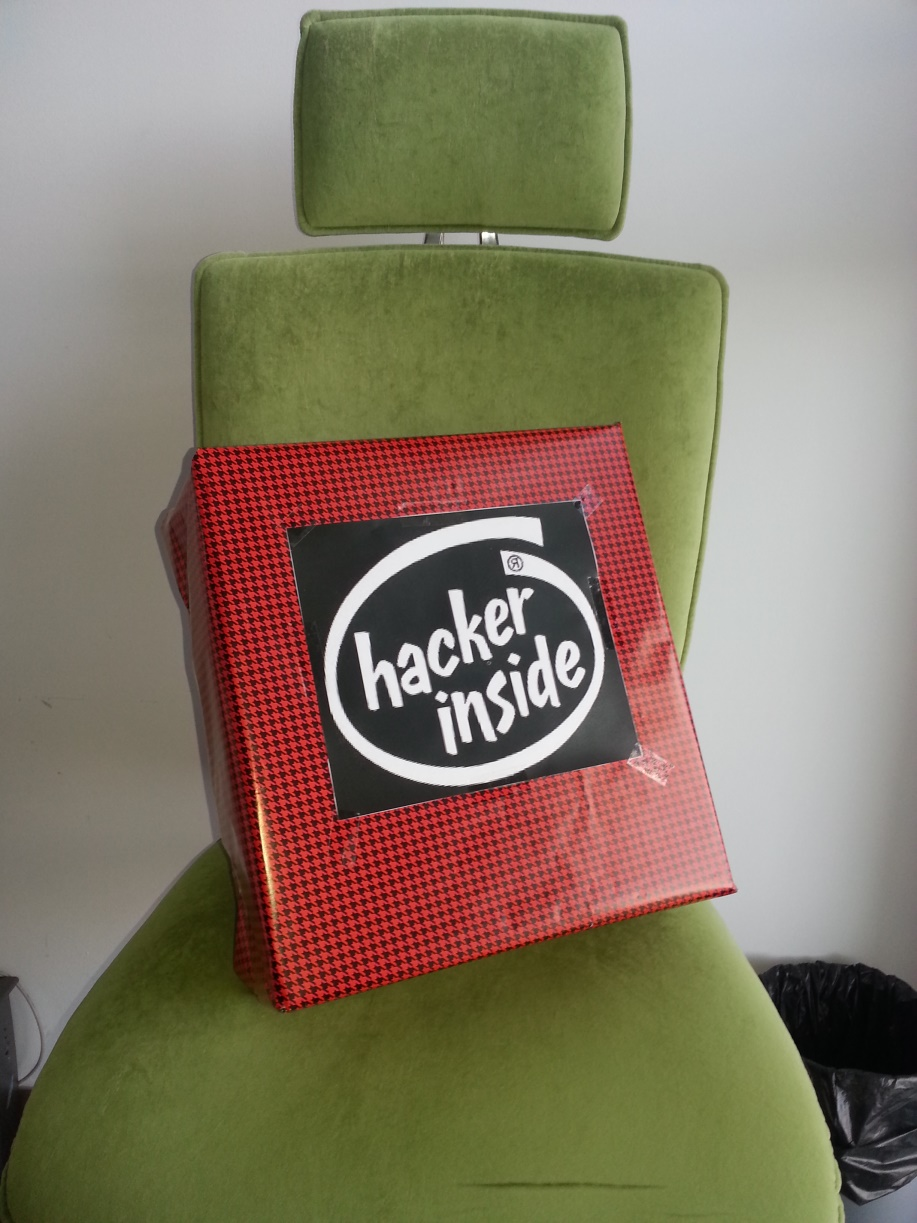
\includegraphics[width=0.21\textwidth]{img/s17_2.jpg}\end{center}
\end{frame}

\begin{frame}[allowframebreaks]{Evaluación}
\small
\begin{itemize}
  \item Ventajas de la convocatoria ordinaria:
  \begin{itemize}
    \item Optas a 11 puntos sobre 10
    \item Si un alumno se presenta según el modo de evaluación continua pero su nota en el examen final es superior a la evaluación continua, la nota final será la del examen
    \item Basado en el histórico, los alumnos que superan la convocatoria continua aprueban toda la asignatura.
    \item Se aprende más y mejor…
  \end{itemize}
  \item Tanto la nota de Teoría como la de Prácticas se guardan para la convocatoria extraordinaria si ésta es superior a 5 puntos.
  \item Sólo se podrá recuperar el Examen Final (teoría y/o prácticas), las notas de la evaluación continua se mantienen de la ordinaria.
\end{itemize}
\end{frame}

\begin{frame}[allowframebreaks]{Bibliografía}
\small
\begin{itemize}
  \item Editorial 0xWord:
  \begin{itemize}
    \item \url{https://0xword.com}
  \end{itemize}
  \item Toda la información referente a la asignatura se publicará en campus virtual
  \begin{itemize}
    \item \url{https://campusvirtual.uclm.es/}
  \end{itemize}
\end{itemize}
\end{frame}

\begin{frame}[allowframebreaks]{Bibliografía}
\small
\begin{itemize}
  \item Laboratorio de Seguridad
  \begin{itemize}
    \item Kali
    \item Metasploitable2
    \item Repositorio máquinas profesor
  \end{itemize}
\end{itemize}
\end{frame}

\begin{frame}[plain]
  \begin{center}
    {\Huge\bfseries\color{uznavy} ¡Gracias!}\\[1em]
    {\large Seguridad en Sistemas Informáticos --- Tema 1.1}
  \end{center}
\end{frame}

\pdfinfo{ /Title () /Author () /Subject () /Keywords () /Creator () /Producer () }
\end{document}
